%-----------------------------------------------
%  Engineer's & Master's Thesis Template
%  Copyleft by Artur M. Brodzki & Piotr Woźniak
%  Warsaw University of Technology, 2019-2022
%-----------------------------------------------

\documentclass[
    bindingoffset=5mm,  % Binding offset
    footnoteindent=3mm, % Footnote indent
    hyphenation=true    % Hyphenation turn on/off
]{src/wut-thesis}

\graphicspath{{tex/img/}} % Katalog z obrazkami.
\addbibresource{bibliografia.bib} % Plik .bib z bibliografią

\facultyeiti    % Wydział Elektroniki i Technik Informacyjnych
\MasterThesis % Praca inżynierska
\langpol % Praca w języku polskim

\begin{document}

%------------------
% Strona tytułowa
%------------------
\instytut{Instytut telekomunikacji}
\kierunek{Telekomunikacja}
\specjalnosc{Teleinformatyka i Zarządzanie w Telekomunikacji}
\title{
    Sworzenie platformy do modelowania i uruchamiania zamkniętych pętli sterowania w Kubernetes
}
\engtitle{
    Creation of a platform for designing and running closed control loops in Kubernetes
}

\author{Andrzej Gawor}
\album{300528}
\promotor{dr inż. Dariusz Bursztynowski}
\date{\the\year}
\maketitle

%-------------------------------------
% Streszczenie po polsku 
%-------------------------------------
\cleardoublepage % Zaczynamy od nieparzystej strony
\abstract
Projekt opisany w niniejszej pracy skupia się na zaproponowaniu oraz przedstawieniu implementacji  architektury platformy, która pozwala na modelowanie oraz uruchamianie zamkniętych pętli sterowania w Kubernetes. Genezą projektu jest praca jednego z komitetów ETSI o nazwie "ENI - Experiential Networked Intelligence", która skupia się na ułatwieniu pracy operatora sieci telekomunikacyjnych wykorzystując mechanizmy sztucznej inteligencji w zamkniętych pętlach sterowania. ENI w jednym ze swoich dokumentów dokonuje przeglądu zamkniętych pętli sterowania znanych ludzkości z innych dziedzin. 

Naturalnym następnym krokiem jest zapropowanie platformy, na której operator mógłby takowe pętle projektować oraz uruchamiać. W tym celu zdefiniowanio zestaw wymagań oraz założeń dla takiego systemu. Jako środowisko uruchomieniowe wybrano  Kubernetes z racji, że jest to system dobrze znany w społeczności oraz sam natywnie używa zamkniętych pętli sterowania. Następnie przeprowadzono obszerną analizę jak za pomocą mechanizmów rozszerzania Kubernetes takich jak "Custom Resources" oraz "Operator" pattern można stworzyć framework umożliwiający modelowanie zamkniętych pętli sterowania. Praca opisuje powstałą platformę, jej architekturę, semantykę składni w definiowanych obiektach, zasady działania, integracje z zewnętrznymi systemami oraz instrukcję jej użytkowania. Omówiona została również implemtacja platformy, technologie za nią stojące oraz decyzje podjęte podczas jej powstawania. Finalnie przedstawiono również test działania platformy w praktyce wykorzystując do tego emulator systemu 5G jakim jest Open5GS w połączeniu z UERANSIM. Pracę podsumuję lista wniosków oraz potencjalnych dróg rozwoju platformy. 
\keywords Zamknięte pętle sterowania, Kubernetes, Zarządzanie sieciami telekomunikacyjnymi, Automatyzacja, Go, Open5GS, Mikroserwisy

%----------------------------------------
% Streszczenie po angielsku
%----------------------------------------
\clearpage
\secondabstract
The project described in this thesis focuses on proposing and implementing a reusable architecture (hereafter referred to as "the Platform") that enables the modeling and execution of closed control loops in Kubernetes. The genesis of the project lies in the work of one of the ETSI committees called "ENI - Experiential Networked Intelligence," which aims to simplify the work of telecommunications network operators by leveraging artificial intelligence mechanisms in closed control loops based on metadata-driven and context-aware policies. In one of its documents, ENI reviews closed control loops known to humanity from other fields. A natural next step is to propose a platform on which operators could design and execute such loops. 

To achieve this, a set of requirements and assumptions for such a system was defined. Kubernetes was chosen as the runtime environment due to its widespread adoption in the community and its inherent use of closed control loops. An extensive analysis was conducted on how Kubernetes extension mechanisms, such as "Custom Resources" and the "Operator" pattern, could be used to create a framework enabling the modeling of closed control loops. 

This thesis describes the developed platform, its architecture, the semantics of syntax in the defined objects, operational principles, integrations with external systems, and a user guide. It also discusses the platform's implementation, the technologies behind it, and the decisions made during its development. Finally, the thesis presents a practical test of the platform's functionality using the Open5GS 5G system emulator in combination with UERANSIM. The work concludes with a list of findings and potential extensions or improvements to the platform.
\secondkeywords Closed Control Loops, Kubernetes, Managing Telco-Networks, Automation, Go, Open5GS, Microservices

\pagestyle{plain}

%--------------
% Spis treści
%--------------
\cleardoublepage % Zaczynamy od nieparzystej strony
\tableofcontents

%------------
% Rozdziały
%------------
\cleardoublepage % Zaczynamy od nieparzystej strony
\pagestyle{headings}
\newpage
\section{Wstęp}
\subsection{Przedmowa}


\subsection{Cel i zakres pracy}

Celem pracy jest kontynuacja badań ENI, polegająca na zaproponowaniu \hyperlink{def:architektura}{\textit{architektury}} platformy, na której możliwe będzie modelowanie oraz uruchamianie zamkniętych pętli sterowania. Niniejsza praca nie skupia się na aspektach związanych ze sztuczną inteligencją. Platforma ma jedynie służyć do zamodelowania oraz uruchomienia \hyperlink{def:workflow}{\textit{workflow}} pętli, ale sama nie stanowi środowiska wykonawczego dla jej komponentów. 

W zakres pracy wchodzi: sformułowanie wymagań na platformę, opracowanie proponowanej architektury wsparte licznymi badaniami podczas jej powstawania, implementacja PoC (ang. \textit{Proof of Concept}) według proponowanej architektury, przeprowadzenie testów platformy oraz analiza jej potencjału w kontekście dalszego rozwoju. Po publikacji praca może stanowić podstawę do implementacji . \hyperlink{def:kognitywny-system-zarzadzania-siecia}{Kognitywnych Systemów Zarządzania Siecią}, zgodnych ze specyfikacjami ENI. 
\subsection{Struktura pracy}

Praca została podzielona na 6 rozdziałów. Drugi rozdział przedstawia bardziej szczegółowo niż we wstępie badania podjęte przez ENI. Stanowi on wprowadzenie teoretyczne oraz pojęciowe, aby ułatwić przekaz w dalszej części pracy. Rozdział trzeci zawiera opis proponowanej architektury. Rozdział czwarty opisuje implementację PoC platformy oraz napotkane wyzwania podczas formułowania architektury, które celowo zostały zebrane w jedno miejsce i umieszczone oddzielnie w celu łatwiejszej lektury. Rozdział numer pięć przedstawia użycie platformy w praktyce przy okazji stanowiąc jej test. Na koniec, w rozdziale szóstym przeprowadzono analizę zaproponowanej architektury, jej możliwości oraz ograniczenia oraz wskazano kierunki potencjalnego rozwoju. 

%---------------
% Literatura
%---------------
\cleardoublepage % Zaczynamy od nieparzystej strony
\printbibliography
\clearpage



%--------------------------------------
% Spisy
%--------------------------------------
\newpage
\pagestyle{plain}
\vspace{0.8cm}
\acronymlist

\hypertarget{def:architektura}{}
\acronym{Architektura}{Zbiór reguł i metod opisujących funkcjonalność, organizację oraz implementację systemu.}

\hypertarget{def:cladra}{}
\acronym{CLADRA}{Closed Loop Anomaly Detection and Resolution Automation}

\hypertarget{def:danae}{}
\acronym{Dane}{Fakty oraz statystyk zebrane razem w celu analizy. Stanowią podstawę do wydobycia z ich \hyperlink{def:informacja}{Informacji}}

\hypertarget{def:custom-resource-definitions}{}
\acronym{Definicje Zasobów Własnych (ang. \textit{Custom Resource Definitions})}{Pliki manifestacyjne YAML służące do zarejestrowania w klastrze nowe zasoby własne}

\hypertarget{def:doswiadczenie}{}
\acronym{Doświadczenie (ang. \textit{Experience})}{Proces zdobywania \hyperlink{def:wiedza}{wiedzy} przez system podczas funkcjonowania w środowisku docelowym}.

\hypertarget{def:edukacja}{}
\acronym{Edukacja (ang. \textit{Education})}{Proces zdobywania \hyperlink{def:wiedza}{wiedzy} przez system poza środowiskiem docelowym, np. podczas trenowania modelu}.

\hypertarget{def:wiedza}{}
\acronym{Wiedza (ang. \textit{Knowledge})}{Zestaw wzorców, które są wykorzystywane do wyjaśniania, a także przewidywania tego, co się wydarzyło, dzieje lub może się wydarzyć w przyszłości. Bazuje na danych, informacjach oraz umiejętnościach zdobytych poprzez \hyperlink{def:doswiadczenie}{doświadczenie} oraz \hyperlink{def:edukacja}{edukację}}

\hypertarget{def:eni}{}
\acronym{ENI}{Experiential Networked Intelligence}

\hypertarget{def:etsi}{}
\acronym{ETSI}{Europen Telecommunications Standards Institute}

\hypertarget{Informacja}{Reprezentacja pojęć będących przedmiotem zainteresowania środowiska w formie niezależnej od formy \hyperlink{def:dane}{danych}}

\hypertarget{def:kognitywnosc}{}
\acronym{Kognitywność (ang. \textit{cognition})}{Proces rozumienia danych oraz informacji w celu produkcji nowych danych, informacji oraz wiedzy}

\hypertarget{def:kognitywny-system-zarzadzania-siecia}{}
\acronym{Kognitywny System Zarządzania Siecią}{System zarządzania siecią, który jest jednocześnie \hyperlink{def:system-kognitywny}{kognitywny}. Docelowy system specyfikowany przez ENI}

\hypertarget{def:kontroler}{}
\acronym{Kontroler (ang. \textit{controller})}{Proces monitorujący stan obiektów API w klastrze i doprowadzający je do stanu pożądanego}

\hypertarget{def:obiekt-api}{}
\acronym{Obiekt API (ang. \textit{API object})}{Zasób reprezentujący element klastra, np. Poda, Deployment, Service. Jest przechowywany w etcd i zarządzany przez API Server. Jest to konkretna instancja danego typu (ang. \textit{Kind}) zasobów}

\hypertarget{def:plik-manifestowy}{}
\acronym{Plik Manifestowy YAML (ang. \textit{YAML Manifest File})}{Plik konfiguracyjny zapisany w formacie YAML, definiujący obiekty API Kubernetes. Służy do deklaratywnego zarządzania zasobami klastra}

\hypertarget{def:polityka}{}
\acronym{Polityka (ang. \textit{Policy})}{Zestaw reguł, który jest używany do zarządzania i kontrolowania zmiany i/lub utrzymania stanu jednego lub więcej zarządzanych obiektów}

\hypertarget{def:regulator}{}
\acronym{Regulator (ang. \textit{Control System})}{Pojęcie z teorii sterowania. System, który reguluje pracę obiektu}

\hypertarget{def:data-driven}{}
\acronym{Sterowany danymi (ang. \textit{Data-Driven})}{Nie narzucający żadnej logiki pętli – logika jest interpretowana na podstawie danych.}

\hypertarget{def:system-eni}{}
\acronym{System ENI}{Centralny punkt architektury ENI. Odpowiedzialny za zamkniętą pętlę sterowania, za pomocą której ENI chce osiągnąć kognitywność. Lupus aspiruje do tego, aby zaproponować architekturę dla Systemu ENI na Kubernetes}

\hypertarget{def:system-kognitywny}{}
\acronym{System kognitywny}{System, który uczy się, wnioskuje oraz podejmuje decyzje w sposób przypominający ludzki umysł}

\hypertarget{def:uczenie-maszynowe}{}
\acronym{Uczenie maszynowe (ang. \textit{Machine Learning})}{proces, który zdobywa nową wiedzę i/lub aktualizuje istniejącą wiedzę w celu optymalizacji funkcjonowanie systemu przy użyciu przykładowych obserwacji}

\hypertarget{def:swiadomosc-kontekstu}{}
\acronym{Świadomość kontekstu (ang. \textit{Context Aware})}{Posiadanie przez system informacji oraz wiedzy, które opisują środowisko w jakim znajduje się dana jednostka w celu lepszego doboru \hyperlink{def:wzorzec}{wzorca} do rozwiązania danego problemu}

\hypertarget{def:wzorzec}{}
\acronym{Wzorzecz (ang. \textit{pattern})}{Generyczne, reużywalne rozwiązanie danego problemu. Część składowa wiedzy}.

\hypertarget{def:warstwa-sterowania}{}
\acronym{Warstwa Sterowania (ang. \textit{Control Plane})}{Zestaw komponentów zarządzających stanem klastra Kubernetes. W szczególności \textsl{Controller Manager}, który nadzoruje kontrolery zasobów}

\hypertarget{def:workflow}{}
\acronym{Workflow}{Sekwencja połączonych węzłów, czasami zależnych warunkowo, która realizuje określony cel. Zazwyczaj workflow definiuje się w celu organizacji pracy.}

\hypertarget{def:wnioskowanie}{}
\acronym{Wnioskowanie (ang. \textit{reasoning})}{Proces, w którym system wyciąga logiczne wnioski z dostępnych danych i wiedzy}

\hypertarget{def:wzorzec-operator}{}
\acronym{Wzorzec Operator (ang. \textit{Operator Pattern})}{Rozszerzenie Kubernetes pozwalające rozwijać kontrolery dla zasobów własnych}

\hypertarget{def:zasoby-wlasne}{}
\acronym{Zasoby Własne (ang. \textit{Custom Resources})}{Mechanizm rozszerzenia klastra Kubernetes o nowe typy obiektów API}

\listoffigurestoc    % Spis rysunków.
\vspace{1cm}         % vertical space
\listoftablestoc     % Spis tabel.
\vspace{1cm}         
\listofappendicestoc % Spis załączników

%-------------
% Załączniki
%-------------
% Obrazki i tabele w załącznikach nie trafiają do spisów
\captionsetup[figure]{list=no}
\captionsetup[table]{list=no}

\appendix{Definicje}\label{appendix:1}

\acronym{Architektura}{Zbiór reguł i metod opisujących funkcjonalność, organizację oraz implementację systemu.}\label{def:architektura}

\acronym{Workflow}{Sekwencja połączonych węzłów, czasami zależnych warunkowo, która realizuje określony cel. Zazwyczaj workflow defniuje się w celu organizacji pracy}\label{def:workflow}
\appendix{Instalacja Lupus}\label{appendix:2}

Specyfikacja w formie elektronicznej znajduje się pod linkiem: \url{https://github.com/0x41gawor/lupus/blob/master/docs/installation.md}.

\subsection{Przedsłowie}

Instalacja \hyperlink{def:lupus}{\textbf{Lupus}} wymaga umiejętności technicznych oraz podstawowej znajomości operacyjnej Kubernetes.

\hyperlink{def:lupus}{\textbf{Lupus}} jest zaimplementowany jako projekt Kubebuilder\footnote{\url{https://book.kubebuilder.io}}. Zalecanym sposobem instalacji \hyperlink{def:lupus}{\textbf{Lupus}} jest sklonowanie tego repozytorium i przyjęcie roli dewelopera tego projektu.

Nie istnieje coś takiego jak instalacja \hyperlink{def:lupus}{\textbf{Lupus}} (np. w systemie operacyjnym). Można zainstalować \hyperlink{def:zasoby-wlasne}{\textbf{Zasoby Własne}} dla \hyperlink{def:element-lupus}{\textbf{Elementów Lupus}} w klastrze Kubernetes i uruchomić dla nich \hyperlink{def:operator-zasobu-element}{\textbf{Kontrolery}}. Niniejszy załącznik opisuje właśnie taki proces.

\subsection{Wymagania wstępne}

\hyperlink{def:uzytkownik}{\textbf{Użytkownik}} musi posiadać działający klaster Kubernetes. Może to być Minikube\footnote{\url{https://minikube.sigs.k8s.io/docs/}}, zainstalowany silnik kontenerów (ang. \textit{container engine}) (np. Docker\footnote{\url{https://docs.docker.com}}) oraz język Go\footnote{\url{https://go.dev}}.

\subsubsection{Instalacja Kubebuilder}

Instrukcja dostępna pod adresem: \url{https://book.kubebuilder.io/quick-start}.

\subsection{Klonowanie repozytorium}

\begin{lstlisting}[language=bash, caption={Klonowanie repozytorium}]
git clone https://github.com/0x41gawor/lupus
cd lupus
\end{lstlisting}

\subsection{Instalacja CRD w klastrze}

To polecenie zastosuje \hyperlink{def:crd}{\textbf{CRD}} (pl. Definicje \hyperlink{def:zasoby-wlasne}{\textbf{Zasobów Własnych}}) dla \hyperlink{def:master}{\textbf{Master}} i \hyperlink{def:element}{\textbf{Element}}, umożliwiając ich użycie.

\begin{lstlisting}[language=bash, caption={Instalacja CRD}]
make install
\end{lstlisting}

\subsection{Uruchomienie kontrolerów }

To polecenie uruchomi \textit{kontrolery} dla \textit{zasobów własnych} \hyperlink{def:master}{\textbf{master}} i \hyperlink{def:element}{\textbf{element}}.

\begin{lstlisting}[language=bash, caption={Uruchomienie kontrolerów}]
make run
\end{lstlisting}

Istnieje możliwość uruchomienia kontrolerów jako pody w klastrze Kubernetes. W tym celu użytkownik jest zaproszony do bliższego zapoznania się z platformą Kubebuilder. Dopóki \hyperlink{def:uzytkownik}{\textbf{Użytkownik}} jest pewien, że nie będzie dopisywał \hyperlink{def:funkcje-uzytkownika}{\textbf{Funkcji Użytkownika}} nie jest to zalecane podejście. 



\appendix{Specyfikacja notacji LupN}\label{appendix:3}

Specyfikacja w formie elektronicznej znajduje się pod linkiem: \url{https://github.com/0x41gawor/lupus/blob/master/docs/spec/lupn.md}.


\hyperlink{def:lupn}{\textbf{LupN}} (od ang. \textit{loop} oraz \textit{Notation}) to język/notacja służąca do wyrażania \hyperlink{def:workflow-petli}{\textbf{Workflow Pętli}}. Nie zawiera opisu \hyperlink{def:czesc-obliczeniowa}{\textbf{Części Obliczeniowej}} \hyperlink{def:logika-petli}{\textbf{Logiki Pętli}}. \hyperlink{def:czesc-obliczeniowa}{\textbf{Część Obliczeniowa}} jest określona poza \hyperlink{def:lupus}{\textbf{Lupus}}, w \hyperlink{def:element-zewnetrzny}{\textbf{Elementach Zewnętrznych}}.

\texttt{LupN} specyfikuje:
\begin{itemize}
    \item \hyperlink{def:workflow-petli}{\textbf{Workflow Pętli}}, czyli workflow \hyperlink{def:element-lupus}{\textbf{Elementów Lupus}},
    \item odniesienia do \hyperlink{def:element-zewnetrzny}{\textbf{Elementów Zewnętrznych}}, wyrażone jako \hyperlink{def:destynacja}{\textbf{Destynacje}},
    \item \hyperlink{def:workflow-petli}{\textbf{Workflow Akcji}} w ramach \hyperlink{def:element-lupus}{\textbf{Elementu Lupus}},
    \item odniesienie (lub odniesienia) do \hyperlink{def:agent-egress}{\textbf{Agenta Egress}} jako \hyperlink{def:destynacja}{\textbf{Destynacja}}.
\end{itemize}

Jak można zauważyć, \texttt{LupN} wyraża \textbf{workflow} na dwóch poziomach: globalnym (czyli \hyperlink{def:workflow-petli}{\textbf{Workflow Elementów Lupus}}) oraz wewnątrz \hyperlink{def:element-lupus}{\textbf{Elementu Lupus}} (czyli \hyperlink{def:workflow-petli}{\textbf{Workflow Akcji}}). Możliwości obu poziomów są do siebie zbliżone, ale ostatecznie różne. Ten załącznik omówi również tę kwestię.


Z punktu widzenia implementacji \hyperlink{def:plik-lupn}{\textbf{Plik LupN}} to w rzeczywistości \textit{YAML manifest file} dla \hyperlink{def:zasoby-wlasne}{\textit{Zasobu Własnego}} \hyperlink{def:master}{\textbf{Master}}. Po zaaplikowaniu (ang. \textit{apply}), \hyperlink{def:operator-zasobu-master}{\textbf{Operator Zasobu Master}} uruchamia \hyperlink{def:element-lupus}{\textbf{Elementy Lupus}}, które realizują wyrażone \hyperlink{def:workflow-petli}{\textbf{Workflow Pętli}}.

\texttt{LupN} wyraża \hyperlink{def:workflow-petli}{\textbf{Workflow Pętli}} poprzez specyfikację różnych obiektów w notacji YAML. Nazwijmy te obiekty \hyperlink{def:obiekt-lupn}{\textbf{Obiektami LupN}}. \hyperref[appendix:3]{Załącznik 3} specyfikuje te obiekty oraz relacje między nimi. Wskazuje również, co oznacza użycie każdego z nich w kontekście \hyperlink{def:workflow-petli}{\textbf{Workflow Pętli}} i jak \hyperlink{def:operator-zasobu-element}{\textbf{Operator Zasobu Element}} je interpretuje w czasie działania.

Okazuje się, że obiekty YAML w \textbf{YAML manifest files} są pochodnymi struktur Golang (typów Golang), dlatego możemy opisać \hyperlink{def:obiekt-lupn}{\textbf{Obiekty LupN}} na podstawie tych struktur Golang. Obiekty YAML w \hyperlink{def:plik-lupn}{\textbf{Pliku LupN}} są pochodnymi struktur Go, dlatego \hyperlink{def:obiekt-lupn}{\textbf{Obiekty LupN}} możemy opisać na ich podstawie. 

Wymagane jest wcześniejsze zapoznanie się z YAML. Załącznik nie obejmuje translacji dokonywanej przez Kubernetes między strukturami Go a reprezentacjami obiektów YAML. Serializacja jest wykonywana przez \texttt{controller-gen} i opisana w \textit{Kubebuilder Book}. Tłumaczenie to można łatwo zaobserwować i nauczyć się, analizując przykłady zamieszczone w repozytorium projektu: \url{https://github.com/0x41gawor/lupus/tree/master/examples}

\subsection{Możliwości LupN}

Ze względu na różnice implementacyjne węzłów omówione w podrozdziale \ref{sec:dwa-rodzaje-workflow}, możliwości \hyperlink{def:workflow-petli}{Workflow Pętli} oraz \hyperlink{def:workflow-akcji}{Workflow Akcji} różnią się od siebie. Sekwencja wykonawcza elementów jest definiowana poprzez obiekty \texttt{next}. Każdy element definiuje listę następnych elementów. Zazwyczaj jest to jeden element. Możliwe są rozgałęzienia (ang. \textit{forks}) czyli lista z większą ilością elementów, ale wtedy zostaje wywołane wiele elementów niezależnie. Nie ma możliwości na zsynchronizowane powrotne złączenie przepływu danych. W przypadku akcji stosowany jest ten sam mechanizm opierający się na definiowaniu następnej akcji, z tym, że tutaj może być ona tylko jedna. Flow akcji interpretowane jest bowiem przez kontroler elementu, który procesuje je po jednej na raz. Z tego powodu możliwe jest sterowanie przepływem (ang. \textit{flow control}), które zostało zaimplementowane jako specjalny typ akcji - \texttt{switch}. 

\subsection{Specyfikacja}

\textbf{Plik LupN} posiada 4 główne pola (ang. \textit{top-level fields}).

\begin{lstlisting}[language=bash, caption={Główne pola pliku LupN}\label{lst:a31}]
apiVersion: lupus.gawor.io/v1
kind: Master
metadata:
  labels:
    app.kubernetes.io/name: lupus
    app.kubernetes.io/managed-by: kustomize
  name: lola
spec:
	<lupn-objects>
\end{lstlisting}

Każde z nich musi być ustawione jak w \ref{lst:a31} oprócz \texttt{metadata.name}, to pole odróżnia instancje pętli między sobą w obrębie klastra Kubernetes.

Notacja LupN rozpoczyna się od pola \texttt{spec}. Każdy obiekt Lupn zostanie opisany poprzez swoją definicję w Go.

\subsubsection{Drzewo obiektów LupN}

Podczas przeglądania specyfikacji \hyperlink{def:obiekt-lupn}{\textbf{obiektów LupN}} pomocne będzie śledzenie aktualnej pozycji w drzewie zależności obiektów. 

\begin{figure}[!h]
    \centering 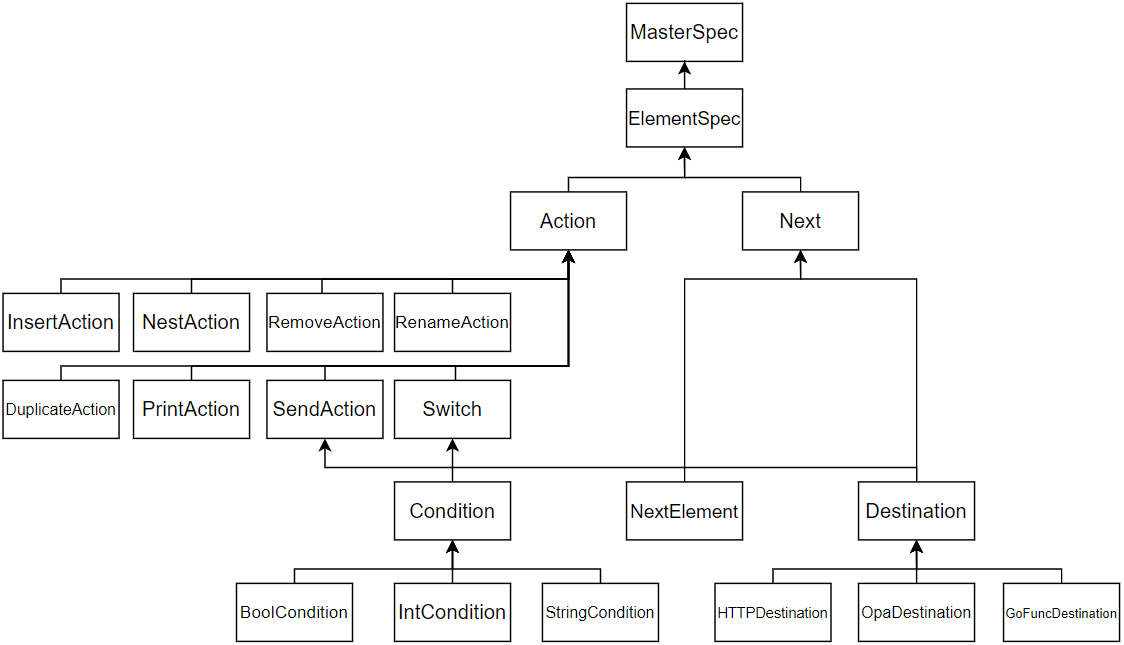
\includegraphics[width=1\linewidth]{a3-tree.png}
    \caption{Drzewko zależności obiektów LupN}\label{fig:a3-tree}
\end{figure}

\subsubsection{MasterSpec}
\begin{lstlisting}[language=go, caption={MasterSpec}\label{lst:a32}]
// MasterSpec defines the desired state of Master
type MasterSpec struct {
	// Name of the Master CR (indicating the name of the loop)
	Name string `json:"name"`
	// Elements is a list of Lupus-Elements
	Elements []*ElementSpec `json:"elements"`
}
\end{lstlisting}
Każdy element na liście \texttt{Elements} spowoduje, że \textbf{Operator Zasobu Master} stworzy obiekt API typu \textbf{Lupus Element}. 

\subsubsection{ElementSpec}
\begin{lstlisting}[language=go, caption={MasterSpec}\label{lst:a32}, basicstyle=\ttfamily\tiny]
// ElementSpec defines the desired state of Element
type ElementSpec struct {
	// Name is the name of the element, its distinct from Kubernetes API Object name, 
    // but rather serves ease of managemenet aspect for loop-designer
	Name string `json:"name"`
	// Descr is the description of the lupus-element, same as Name it serves as 
    // the ease of management aspect for loop-designer
	Descr string `json:"descr"`
	// Actions is a list of Actions that lupus-element has to perform
	Actions []Action `json:"actions,omitempty"`
	// Next is a list of next objects (can be lupus-element or external-element) 
    // to which send the final-data
	Next []Next `json:"next,omitempty"`
	// Name of master element (used as prefix for lupus-element name)
	Master string `json:"master,omitempty"`
}
\end{lstlisting}

\subsubsection{Next}
\begin{lstlisting}[language=go, caption={Next}\label{lst:next}, basicstyle=\ttfamily\tiny]
// Next specifies the next loop-element in a loop workflow, 
// it may be either lupus-element or reference to an external-element
// It allows to forward the whole final-data, but also parts of it
type Next struct {
	// Type specifies the type of next loop-element, lupus-element (element) 
    // or external-element (destination)
	Type string `json:"type" kubebuilder:"validation:Enum=element,destination"`
	// List of input keys (Data fields) that have to be forwarded
	// Pass array with single element '*' to forward the whole input
	Keys []string `json:"keys"`
	// One of the fields below is not null
	Element     *NextElement `json:"element,omitempty" kubebuilder:"validation:Optional"`
	Destination *Destination `json:"destination,omitempty" kubebuilder:"validation:Optional"`
}
\end{lstlisting}

\subsubsection{NextElement}
\begin{lstlisting}[language=go, caption={NextElement}\label{lst:nextelement}]
// NextElement indicates the next loop-element 
// in loop-workflow of type lupus-element
type NextElement struct {
	// Name is the lupus-name of lupus-element 
	// (the one specified in Element struct)
	Name string `json:"name"`
}
\end{lstlisting}

\subsubsection{Destination}
\begin{lstlisting}[language=go, caption={Destination}\label{lst:destination}, basicstyle=\ttfamily\tiny]
// Destination represents an external-element
// It holds all the info needed to make a call to an external-element
// It supports calls to HTTP server, Open Policy Agent or user-functions
type Destination struct {
	// Type specifies if the external element is: a HTTP server in general, 
    // a special kind of HTTP server like Open Policy Agent or internal, a user-function
	Type string `json:"type" kubebuilder:"validation:Enum=http;opa;gofunc"`
	// One of these fields is not null depending on a Type
	HTTP   *HTTPDestination   `json:"http,omitempty" kubebuilder:"validation:Optional"`
	Opa    *OpaDestination    `json:"opa,omitempty" kubebuilder:"validation:Optional"`
	GoFunc *GoFuncDestination `json:"gofunc,omitempty" kubebuilder:"validation:Optional"`
}
\end{lstlisting}

\subsubsection{HTTPDestination}
\begin{lstlisting}[language=go, caption={HTTPDestination}\label{lst:httpdestination}]
// HTTPDestination defines fields specific to a HTTP type
// This is information needed to make a HTTP request
type HTTPDestination struct {
	// Path specifies HTTP URI
	Path string `json:"path"`
	// Method specifies HTTP method
	Method string `json:"method"`
}
\end{lstlisting}

\subsubsection{OpaDestination}
\begin{lstlisting}[language=go, caption={OpaDestination}\label{lst:opadestination}]
// OpaDestination defines fields specific to Open Policy Agent type
// This is information needed to make an Open Policy Agent request
// Call to Opa is actually a special type of HTTP call
type OpaDestination struct {
	// Path specifies HTTP URI, since method is known
	Path string `json:"path"`
}
\end{lstlisting}

\subsubsection{GoFuncDestination}
\begin{lstlisting}[language=go, caption={GoFuncDestination}\label{lst:gofuncdestination}]
// GoFuncDestination defines fields specific to GoFunc type
// This is information needed to call an user-function
type GoFuncDestination struct {
	// Name specifies the name of the function
	Name string `json:"name"`
}
\end{lstlisting}

\subsubsection{Action}
\begin{lstlisting}[language=go, caption={Action}\label{lst:action}, basicstyle=\ttfamily\tiny]
// Action represents operation that is performed on Data
// Action is used in Element spec. Element has a list of Actions 
// and executes them in a workflow manner
// In general, each action has an input and output keys that define 
// which Data fields it has to work on
// Each action indicates the name of the next Action in Action Chain
// There is special type - Switch. Actually, it does not perform any operation on Data, 
// but rather controls the flow of Actions chain
type Action struct {
	// Name of the Action, it is for designer to ease the management of the Loop
	Name string `json:"name"`
	// Type of Action
	Type string `json:"type" kubebuilder:"validation:Enum=send,nest,remove,rename,duplicate,print,insert,switch"`
	// One of these fields is not null depending on a Type.
	Send      *SendAction      `json:"send,omitempty" kubebuilder:"validation:Optional"`
	Nest      *NestAction      `json:"nest,omitempty" kubebuilder:"validation:Optional"`
	Remove    *RemoveAction    `json:"remove,omitempty" kubebuilder:"validation:Optional"`
	Rename    *RenameAction    `json:"rename,omitempty" kubebuilder:"validation:Optional"`
	Duplicate *DuplicateAction `json:"duplicate,omitempty" kubebuilder:"validation:Optional"`
	Print     *PrintAction     `json:"print,omitempty" kubebuilder:"validation:Optional"`
	Insert    *InsertAction    `json:"insert,omitempty" kubebuilder:"validation:Optional"`
	Switch    *Switch          `json:"switch,omitempty" kubebuilder:"validation:Optional"`
	// Next is the name of the next action to execute, in the case of Switch-type action it stands as a default branch
	Next string `json:"next"`
}
\end{lstlisting}

Pole \texttt{Next}, oprócz nazw akcji, może przyjąć jedną z dwóch zdefiniowanych wartości. Wartość \texttt{final} oznacza, że postać \hyperlink{def:dane}{\textbf{Danych}} po tej akcji jest już w swojej \hyperlink{def:finalne-dane}{\textbf{Finalnej Postaci}} i musi zostać przekazana do następnego \hyperlink{def:element-lupus}{\textbf{Elementu Lupus}}. Wartość \texttt{exit} oznacza nagłe zaniechanie aktualnej iteracji \hyperlink{def:zamknieta-petla-sterowania}{\textbf{Pętli Sterowania}} (zazwyczaj wskutek błędu).

\subsubsection{SendAction}
\begin{lstlisting}[language=go, caption={SendAction}\label{lst:sendaction}]
// SendAction is used to make call to external-element
// Element's controller obtains a data field using InputKey,
// and attaches it as a json body when performing a call to destination.
// Response is saved in data under an OutputKey
type SendAction struct {
	InputKey    string      `json:"inputKey"`
	Destination Destination `json:"destination"`
	OutputKey   string      `json:"outputKey"`
}
\end{lstlisting}

\subsubsection{InsertAction}
\begin{lstlisting}[language=go, caption={InsertAction}\label{lst:insertaction}]
// InsertAction is used to make a new field and insert value to it
// Normally new fields are created as an outcome of other types of actions
// It is useful in debugging or logging, 
// e.g. can indicate the path taken by the actions workflow
type InsertAction struct {
	OutputKey string               `json:"outputKey"`
	Value     runtime.RawExtension `json:"value"`
}
\end{lstlisting}

\subsubsection{NestAction}
\begin{lstlisting}[language=go, caption={NestAction}\label{lst:nestaction}]
// NestAction is used to group a number of data-fields together.
// Element's controllers gather fields indicated by InputKeys list
// and nest them in a new field under an OutputKey.
type NestAction struct {
	InputKeys []string `json:"inputKeys"`
	OutputKey string   `json:"outputKey"`
}
\end{lstlisting}

\subsubsection{RemoveAction}
\begin{lstlisting}[language=go, caption={RemoveAction}\label{lst:removeaction}]
// RemoveAction is used to delete a data-field.
// Elements' controllers remove fields indicated by the list InputKeys
type RemoveAction struct {
	InputKeys []string `json:"inputKeys"`
}
\end{lstlisting}

\subsubsection{RenameAction}
\begin{lstlisting}[language=go, caption={RenameAction}\label{lst:renameaction}]
// RenameAction is used to change the name of a data-field.
// InputKey indicates a field to be renamed
// OutputKey is the new field name.
type RenameAction struct {
	InputKey  string `json:"inputKey"`
	OutputKey string `json:"outputKey"`
}
\end{lstlisting}

\subsubsection{DuplicateAction}
\begin{lstlisting}[language=go, caption={DuplicateAction}\label{lst:duplicateaction}]
// DuplicateAction is used to make a copy of a data-field.
// InputKey indicates the field of which value has to be copied.
// OutputKey indicates the field to which values have to be pasted in.
type DuplicateAction struct {
	InputKey  string `json:"inputKey"`
	OutputKey string `json:"outputKey"`
}
\end{lstlisting}

\subsubsection{PrintAction}
\begin{lstlisting}[language=go, caption={PrintAction}\label{lst:printaction}]
// PrintAction is used to print the value of each field 
// indicated by InputKeys in a controller's console.
// It is useful in debugging or logging.
type PrintAction struct {
	InputKeys []string `json:"inputKeys"`
}
\end{lstlisting}

\subsubsection{Switch}
\begin{lstlisting}[language=go, caption={Switch}\label{lst:switch}]
// Switch is a special type of action used for flow-control
// When Element's controller encounters switch action on the chain
// it emulates the work of a switch known in other programming languages
type Switch struct {
	Conditions []Condition `json:"conditions"`
}
\end{lstlisting}

\subsubsection{Condition}
\begin{lstlisting}[language=go, caption={Condition}\label{lst:condition}, basicstyle=\ttfamily\tiny]
// Condition represents a single condition present in Switch action
// It defines on which Data field it has to be performed, 
// the actual condition to be evaluated,
// and the next Action if evaluation returns true.
type Condition struct {
	// Key indicates the Data field that has to be retrieved
	Key string `json:"key"`
	// Operator defines the comparison operation, e.g. eq, ne, gt, lt
	Operator string `json:"operator" kubebuilder:"validation:Enum=eq,ne,gt,lt"`
	// Type specifies the type of the value: string, int, float, bool
	Type string `json:"type" kubebuilder:"validation:Enum=string,int,float,bool"`
	// One of these fields is not null depending on a Type.
	BoolCondition   *BoolCondition   `json:"bool,omitempty" kubebuilder:"validation:Optional"`
	IntCondition    *IntCondition    `json:"int,omitempty" kubebuilder:"validation:Optional"`
	StringCondition *StringCondition `json:"string,omitempty" kubebuilder:"validation:Optional"`
	// Next specifies the name of the next action to execute if evaluation returns true
	Next string `json:"next"`
}
\end{lstlisting}

\subsubsection{BoolCondition}
\begin{lstlisting}[language=go, caption={BoolCondition}\label{lst:boolcondition}]
// BoolCondition defines a boolean-specific condition
type BoolCondition struct {
	Value bool `json:"value"`
}
\end{lstlisting}

\subsubsection{IntCondition}
\begin{lstlisting}[language=go, caption={IntCondition}\label{lst:intcondition}]
// IntCondition defines an integer-specific condition
type IntCondition struct {
	Value int `json:"value"`
}
\end{lstlisting}

\subsubsection{StringCondition}
\begin{lstlisting}[language=go, caption={StringCondition}\label{lst:stringcondition}]
// StringCondition defines a string-specific condition
type StringCondition struct {
	Value string `json:"value"`
}
\end{lstlisting}

\appendix{Specyfikacja interfejsów Lupus}\label{appendix:4}

Specyfikacja w formie elektronicznej znajduje się pod linkiem: \url{https://github.com/0x41gawor/lupus/blob/master/docs/spec/lupin-lupout.md}.

\subsection{Architektura}

\begin{figure}[!h]
    \centering 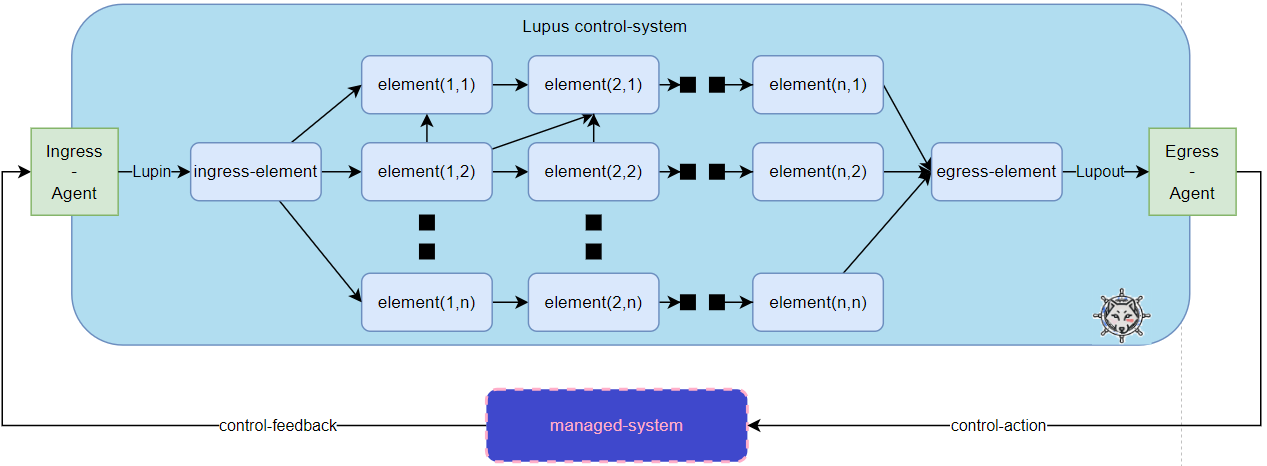
\includegraphics[width=1\linewidth]{a4-arch.png}
    \caption{Architektura Lupus}\label{fig:a4-arch}
\end{figure}

\subsection{Interfejs Lupin}

Projektant może zdefiniować wiele \textbf{Elementów Lupus}, połączonych na różne, skomplikowane sposoby. Musi jednak zdecydować, który z nich zostanie wywołany przez \textbf{IAgenta Ingress}. Taki element można nazwać \textbf{Element Ingress}. Lupus zaleca posiadanie tylko jednego Elementu Ingress.
Jeśli \textbf{Agent Ingress} chce zasygnalizować, że można zaobserwować nowy stan systemu zarządzanego (co oznacza, że musi zostać uruchomiona nowa iteracja pęli sterowania), musi zmodyfikować pole \texttt{Status.Input} w \textit{obiekcie API} \textbf{Elementu Ingress}. Wartość umieszczona w tym polu będzie reprezentować nowy \textbf{Aktualny Stan}.

Pole \texttt{Status.Input} w \textbf{Ingress Element CR} jest typu \texttt{RawExtension}, co oznacza, że podlega pod specyfikacje danych \\TODO załącznik daty

JSON przesłany w tym miejscu będzie stanowił \textbf{Dane} dla tego elementu.

Oprogramowanie implementuje interfejs \texttt{Lupin}, jeśli w pewnym miejscu swojego kodu wysyła żądanie HTTP do \textbf{kube-api-server}, które aktualizuje status \textbf{Elementu Ingress}, a dokładniej pole \texttt{input}. Wartość musi być obiektem JSON, który reprezentuje \textbf{Aktualny Stan} \textbf{Zarządzanego Systemu}. 

\subsection{Interfejs Lupout}

Punktem wyjścia z \textbf{Systemu Sterowania Lupus} jest ostatni \textbf{Element Lupus} czyli (\textbf{Element Egress}). Wysyła on swoje \textbf{finalne dane} (lub ich część) do \textbf{Agenta Egress}. \textbf{Egress Agent} musi przekształcić to wejście w \textbf{Akcje Sterowania}, wykonywaną bezpośrednio na \textbf{systemie zarządzanym}.

Oprogramowanie implementuje interfejs \texttt{Lupout}, jeśli implementuje serwer HTTP, który akceptuje wejściowe dane JSON i tłumaczy je na \textbf{Akcje Sterowania} wykonywaną na \textbf{Systemie Zarządzanym}. 


\appendix{Specfyfikacju obiektu danych}\label{appendix:5}

Specyfikacja w formie elektronicznej znajduje się pod linkiem: \url{https://github.com/0x41gawor/lupus/blob/master/docs/spec/data.md}.

Data jest kluczowym elementem spełnienia \hyperref[req:5]{Wymagania 5}. \textbf{Dane} jest to sposób w jaki \textbf{użytkownik}, podczas każdej iteracji, może:
\begin{itemize}
    \item uzyskać informacje o \textbf{Aktualnym Stanie}
    \item przechowywać pomocnicze informacje (takie jak odpowiedzi od \textbf{Elementów Zewnętrznych})
    \item przechowywać informacje debuggingowe
    \item zapisywać informacje potrzebne do sformułowania \textbf{Akcji Sterowania}
\end{itemize}

\textbf{Dane} są reprezentowane jako JSON dający się zapisać w strukturze Go \texttt{map[string]interface{}}. Nie może, więc być jedną z następujących form obiektu JSON:
\begin{itemize}
    \item typem prymitywnym,
    \item tablicą,
    \item obiektem JSON z kluczami innymi niż string.
\end{itemize}

To w jaki sposób można operować na danych prezentuje specyfikacja akcji //TODO link.
\appendix{Specyfikacja akcji}\label{appendix:6}

Specyfikacja w formie elektronicznej znajduje się pod linkiem: \url{https://github.com/0x41gawor/lupus/blob/master/docs/spec/actions.md}.

Specyfikacja akcji w LupN znajduje się w załączniku //TODO. Ten dokument prezentuje przykładowe działanie \textbf{akcji} na \textbf{danych}.

Akcje zostały opracowane jako najbardziej atomowe operacje, które, gdy zostaną odpowiednio połączone, stanowią narzędzie umożliwiające \textbf{designer'owi pętli} pełne operowanie na \textbf{danych}.

Czasami operacja, która na pierwszy rzut oka wydaje się atomowa, wymaga użycia dwóch połączonych akcji. Z drugiej strony, zdarza się, że operacja początkowo uznana za atomową okazuje się jedynie szczególnym przypadkiem bardziej ogólnej operacji. Dobrym przykładem jest nieistniejąca już akcja \texttt{concat}. Została ona zaprojektowana do łączenia dwóch pól w jedno, jednak okazało się, że jest to specyficzny przypadek akcji \texttt{nest}, w której lista \texttt{InputKey} zawiera tylko dwa elementy.

\subsection{Podział ogólny}

Mamy 8 typów akcji:

\begin{itemize}
    \item \textbf{Send}
    \item \textbf{Nest}
    \item \textbf{Remove}
    \item \textbf{Rename}
    \item \textbf{Duplicate}
    \item \textbf{Insert}
    \item \textbf{Print}
    \item \textbf{Switch}
\end{itemize}

Możemy wyróżnić następujące kategorie:

\begin{itemize}
    \item 6 akcji, które mogą być używane do modyfikacji danych: \\ 
          \texttt{\{Send, Nest, Remove, Rename, Duplicate, Insert\}}
    \item 1 akcja do komunikacji z \textbf{Elementami Zewnętrznymi}: \\ 
          \texttt{\{Send\}}
    \item 2 akcje do debugowania: \\ 
          \texttt{\{Insert, Print\}}
    \item 1 akcja do logowania: \\ 
          \texttt{\{Print\}}
    \item 1 akcja do sterowania przepływem \textbf{workflow akcji}: \\ 
          \texttt{\{Switch\}}
\end{itemize}

\appendix{Kod Agenta Ingress}\hypertarget{appendix:7}{}

Kod w wersji elektronicznej znajduje się pod linkiem: \url{https://github.com/0x41gawor/lupus/blob/master/examples/open5gs/sample-loop/ingress-agent.py}

\begin{lstlisting}[language=python, basicstyle=\ttfamily\tiny, caption={\emph{Kod Agenta Ingress}}\label{lst:a71}]
from kubernetes import client, config
import argparse
import time
import json
from datetime import datetime
import subprocess  
from kubernetes.client import CustomObjectsApi  
from flask import Flask, request, jsonify
from threading import Thread

# Load Kubernetes configuration
config.load_kube_config()

# Kubernetes API clients
core_v1_api = client.CoreV1Api()
apps_v1_api = client.AppsV1Api()

import logging
log = logging.getLogger('werkzeug')
log.setLevel(logging.ERROR)

global interval
round = 0

def get_pods_by_deployment_prefix(prefix):
    try:
        # List all deployments in the current namespace
        deployments = apps_v1_api.list_deployment_for_all_namespaces(watch=False)
        matching_deployments = [d for d in deployments.items if d.metadata.name.startswith(prefix)]
        # Find all pods associated with matching deployments
        pods = core_v1_api.list_pod_for_all_namespaces(watch=False)
        deployment_pod_map = {}
        for deployment in matching_deployments:
            filtered_pods = []
            for pod in pods.items:
                if pod.metadata.owner_references:
                    for owner in pod.metadata.owner_references:
                        if owner.kind == "ReplicaSet" and owner.name.startswith(deployment.metadata.name):
                            filtered_pods.append(pod)
            deployment_pod_map[deployment.metadata.name] = filtered_pods
        
        return deployment_pod_map
    except client.rest.ApiException as e:
        print(f"Exception when calling Kubernetes API: {e}")
        return {}

def get_pod_resources(pod):
    containers = pod.spec.containers
    resource_info = []
    for container in containers:
        resources = container.resources
        resource_info.append({
            "container_name": container.name,
            "requests": resources.requests or {},
            "limits": resources.limits or {},
        })
    return resource_info

def get_pod_actual_usage(pod_name, namespace):
    try:
        # Use kubectl top to fetch actual usage (requires metrics-server installed)
        result = subprocess.run(
            ["kubectl", "top", "pod", pod_name, "-n", namespace, "--no-headers"],
            stdout=subprocess.PIPE,
            stderr=subprocess.PIPE,
            text=True
        )
        if result.returncode == 0:
            usage_data = result.stdout.strip().split()
            if len(usage_data) >= 3:
                return {
                    "cpu": usage_data[1],
                    "memory": usage_data[2],
                }
        else:
            print(f"Error fetching actual usage for pod {pod_name}: {result.stderr}")
            return {}
    except Exception as e:
        print(f"Error running kubectl top for pod {pod_name}: {e}")
        return {}

def get_json_data():
    deployment_prefix = "open5gs-upf"
    deployment_pod_map = get_pods_by_deployment_prefix(deployment_prefix)
    metrics = {}

    for deployment_name, pods in deployment_pod_map.items():
        # Initialize deployment entry in metrics
        metrics[deployment_name] = {
            "requests": {},
            "limits": {},
            "actual": {}
        }


        for pod in pods:
            pod_name = pod.metadata.name
            namespace = pod.metadata.namespace

            # Resource requests and limits
            resource_info = get_pod_resources(pod)
            for container_info in resource_info:
                metrics[deployment_name]["requests"] = container_info["requests"]
                metrics[deployment_name]["limits"] = container_info["limits"]

            # Actual resource usage
            actual_usage = get_pod_actual_usage(pod_name, namespace)
            metrics[deployment_name]["actual"] = actual_usage
    
    return json.dumps(metrics)

def send_to_kube(state):
    custom_objects_api = CustomObjectsApi()  # Use CustomObjectsApi to interact with CRDs
    try:
        # Retrieve the custom resource
        observe = custom_objects_api.get_namespaced_custom_object(
            group="lupus.gawor.io",
            version="v1",
            namespace='default',
            plural="elements",
            name='lola-demux'
        )
        
        # Update the `status.input` field with the state
        observe_status = observe.get('status', {})
        observe_status['input'] = json.loads(state)  # Convert JSON string to an object
        observe_status['lastUpdated'] = datetime.utcnow().isoformat() + "Z"  # Proper ISO 8601 format

        # Update the custom resource's status
        custom_objects_api.patch_namespaced_custom_object_status(
            group="lupus.gawor.io",
            version="v1",
            namespace='default',
            plural="elements",
            name='lola-demux',
            body={"status": observe_status}  # Send only the `status` field
        )
        print("Updated Kubernetes custom resource status successfully.")
    except Exception as e:
        print(f"Error updating custom resource: {e}")

def periodic_task():
    json_data = get_json_data()
    timestamp = datetime.utcnow().strftime('%Y/%m/%d %H:%M:%S')
    global round 
    round = round + 1
    print(timestamp + " Round: " + str(round) + "\n" + json_data)
    send_to_kube(json_data)

app = Flask(__name__)

@app.route('/api/interval', methods=['POST'])
def update_interval():
    global interval
    try:
        data = request.get_json()
        if "value" in data and isinstance(data["value"], int) and data["value"] > 0:
            interval = data["value"]
            return jsonify({"message": "Interval updated successfully", "new_interval": interval}), 200
        else:
            return jsonify({"error": "Invalid input. 'value' must be a positive integer."}), 400
    except Exception as e:
        return jsonify({"error": str(e)}), 500

if __name__ == "__main__":
    parser = argparse.ArgumentParser(description='Periodic K8s metrics fetcher')
    parser.add_argument('--interval', type=int, default=60, help='Interval in seconds for periodic task')
    args = parser.parse_args()
    
    # Declare that you are modifying the global variable
    interval = args.interval

    # Start Flask server in a separate thread
    flask_thread = Thread(target=lambda: app.run(host='0.0.0.0', port=9000, debug=False, use_reloader=False))
    flask_thread.daemon = True
    flask_thread.start()
    
    while True:
        periodic_task()
        time.sleep(interval)
\end{lstlisting}
\appendix{Kod Agenta Egress}\hypertarget{appendix:8}{}

Kod w wersji elektronicznej znajduje się pod linkiem: \url{https://github.com/0x41gawor/lupus/blob/master/examples/open5gs/sample-loop/egress-agent.py}

\begin{lstlisting}[language=python, basicstyle=\ttfamily\tiny, caption={\emph{Kod Agenta Egress}}\label{lst:a81}]
from flask import Flask, request, jsonify
from kubernetes import client, config
from kubernetes.client.rest import ApiException

app = Flask(__name__)

# Load Kubernetes config (use kubeconfig if running locally, in-cluster config if running in a cluster)
try:
    config.load_incluster_config()
except:
    config.load_kube_config()

# Function to patch deployment resources
def patch_deployment_resources(namespace, deployment_name, resource_type, cpu, memory):
    try:
        api_instance = client.AppsV1Api()

        # Define the patch
        patch = {
            "spec": {
                "template": {
                    "spec": {
                        "containers": [
                            {
                                "name": "upf",
                                "resources": {
                                    resource_type.split(".")[-1]: {  # Extract "requests" or "limits"
                                        "cpu": cpu,
                                        "memory": memory
                                    }
                                }
                            }
                        ]
                    }
                }
            }
        }

        # Patch the deployment
        api_response = api_instance.patch_namespaced_deployment(name=deployment_name, namespace=namespace, body=patch)
        return api_response

    except ApiException as e:
        return str(e)

import requests

def send_interval_request(url: str, value: int):
    headers = {
        "Content-Type": "application/json"
    }
    data = {
        "value": value
    }
    try:
        response = requests.post(url, json=data, headers=headers)
        response.raise_for_status()  # Raise an exception for HTTP errors
        return response.json()
    except requests.RequestException as e:
        print(f"Request failed: {e}")
        return None



@app.route('/api/data', methods=['POST'])
def get_data():
    data = request.get_json()
    print(data)
    if "spec" in data:
        deployment_name = data.get('name')
        namespace = 'open5gs'
        lim_cpu = data['spec']['limits'].get('cpu')
        lim_ram = data['spec']['limits'].get('memory')
        req_cpu = data['spec']['requests'].get('cpu')
        req_ram = data['spec']['requests'].get('memory')
        res1 = patch_deployment_resources(namespace, deployment_name, 'resources.limits', lim_cpu, lim_ram)
        res2 = patch_deployment_resources(namespace, deployment_name, 'resources.requests', req_cpu, req_ram)

    if "interval" in data:
        interval = data['interval']
        response = send_interval_request("http://192.168.56.112:9000/api/interval", interval)
    
    return jsonify({"res": "ok"})

if __name__ == '__main__':
    app.run(host='0.0.0.0', port=9001)
\end{lstlisting}
\appendix{Kod Elementów Zewnętrznych}\hypertarget{appendix:9}{}

Kod w wersji elektronicznej znajduje się pod linkiem: \url{https://github.com/0x41gawor/lupus/blob/master/examples/open5gs/sample-loop/opa.py}

\begin{lstlisting}[language=python, basicstyle=\ttfamily\tiny, caption={\emph{Kod Elementów Zewnętrznych}}\label{lst:a91}]
from flask import Flask, request, jsonify

app = Flask(__name__)

# Hardcoded default values
DEFAULT_VALUES = {
    "requests": {
        "memory": "128Mi",
        "cpu": "100m"
    },
    "limits": {
        "memory": "256Mi",
        "cpu": "250m"
    }
}

# ------------------ Parsing Helpers ------------------ #
def parse_cpu(cpu_str: str) -> int:
    """
    Convert a CPU string to an integer representing millicores.
    
    Examples:
      "300m"  -> 300
      "2"     -> 2000  (interpreted as 2 CPU cores -> 2000 millicores)
      "1.5"   -> 1500
    """
    cpu_str = cpu_str.strip().lower()
    if cpu_str.endswith("m"):
        # e.g. "300m" -> 300
        numeric_part = cpu_str[:-1]  # remove "m"
        return int(float(numeric_part))
    else:
        # e.g. "2" -> 2000, "1.5" -> 1500
        return int(float(cpu_str) * 1000)


def parse_memory(mem_str: str) -> int:
    """
    Convert a memory string to an integer representing megabytes (MB).
    
    Examples:
      "300Mi" -> 300
      "1Gi"   -> 1024
      "1024Ki"-> 1
      "512"   -> 512   (no unit, assume MB)
    """
    mem_str = mem_str.strip()
    lower_str = mem_str.lower()

    if lower_str.endswith("mi"):
        # e.g. "300Mi"
        numeric_part = lower_str.replace("mi", "")
        return int(float(numeric_part))
    elif lower_str.endswith("gi"):
        # e.g. "2Gi" -> 2 * 1024 = 2048
        numeric_part = lower_str.replace("gi", "")
        return int(float(numeric_part) * 1024)
    elif lower_str.endswith("ki"):
        # e.g. "1024Ki" -> 1024 / 1024 = 1
        numeric_part = lower_str.replace("ki", "")
        return int(float(numeric_part) / 1024)
    else:
        # e.g. "512" -> 512
        return int(float(lower_str))

# ------------------ Comparison Helpers ------------------ #

def is_higher_cpu(actual_cpu_str, default_cpu_str) -> bool:
    """Return True if actual_cpu_str is higher than default_cpu_str (in millicores)."""
    return parse_cpu(actual_cpu_str) > parse_cpu(default_cpu_str)

def is_higher_memory(actual_mem_str, default_mem_str) -> bool:
    """Return True if actual_mem_str is higher than default_mem_str (in MB)."""
    return parse_memory(actual_mem_str) > parse_memory(default_mem_str)

def is_default_cpu(actual_cpu_str, default_cpu_str) -> bool:
    """Return True if actual == default (in millicores)."""
    return parse_cpu(actual_cpu_str) == parse_cpu(default_cpu_str)

def is_default_memory(actual_mem_str, default_mem_str) -> bool:
    """Return True if actual == default (in MB)."""
    return parse_memory(actual_mem_str) == parse_memory(default_mem_str)

# ------------------ Core Logic ------------------ #
def determine_point(data):
    """
    Determine the operational point type:
    
    1. NORMAL
       - actual < default_values['requests'] for both cpu, memory

    2. NORMAL_TO_CRITICAL
       - requests == default_values['requests']
       - limits == default_values['limits']
       - actual > default_values['requests'] for cpu or memory

    3. CRITICAL
       - actual, requests, limits are ALL higher than the defaults
         (at least one field of each is higher than the default)

    4. CRITICAL_TO_NORMAL
       - requests, limits are above their defaults
       - actual is below the default (requests) for both cpu, memory
    """
    # Extract input values
    req_cpu_str    = data["requests"]["cpu"]
    req_mem_str    = data["requests"]["memory"]
    lim_cpu_str    = data["limits"]["cpu"]
    lim_mem_str    = data["limits"]["memory"]
    act_cpu_str    = data["actual"]["cpu"]
    act_mem_str    = data["actual"]["memory"]

    # Extract defaults
    def_req_cpu = DEFAULT_VALUES["requests"]["cpu"]
    def_req_mem = DEFAULT_VALUES["requests"]["memory"]
    def_lim_cpu = DEFAULT_VALUES["limits"]["cpu"]
    def_lim_mem = DEFAULT_VALUES["limits"]["memory"]

    # 1. NORMAL: actual < default_values.requests (cpu & mem)
    condition_normal = (not is_higher_cpu(act_cpu_str, def_req_cpu) and
                        not is_higher_memory(act_mem_str, def_req_mem))

    # 2. NORMAL_TO_CRITICAL:
    #    - requests == default (cpu & mem)
    #    - limits == default (cpu & mem)
    #    - actual > default.requests for cpu or memory
    condition_normal_to_critical = (
        is_default_cpu(req_cpu_str, def_req_cpu) and
        is_default_memory(req_mem_str, def_req_mem) and
        is_default_cpu(lim_cpu_str, def_lim_cpu) and
        is_default_memory(lim_mem_str, def_lim_mem) and
        (
            is_higher_cpu(act_cpu_str, def_req_cpu) or
            is_higher_memory(act_mem_str, def_req_mem)
        )
    )

    # 3. CRITICAL:
    #    - actual is higher than default requests (cpu or mem)
    #    - requests is higher than default requests (cpu or mem)
    #    - limits is higher than default limits (cpu or mem)
    condition_critical = (
        (is_higher_cpu(act_cpu_str, def_req_cpu) or is_higher_memory(act_mem_str, def_req_mem)) and
        (is_higher_cpu(req_cpu_str, def_req_cpu) or is_higher_memory(req_mem_str, def_req_mem)) and
        (is_higher_cpu(lim_cpu_str, def_lim_cpu) or is_higher_memory(lim_mem_str, def_lim_mem))
    )

    # 4. CRITICAL_TO_NORMAL:
    #    - requests, limits are above defaults
    #    - actual is below default.requests for cpu & mem
    #    => requests > default, limits > default, actual < default
    condition_critical_to_normal = (
        (is_higher_cpu(req_cpu_str, def_req_cpu) or is_higher_memory(req_mem_str, def_req_mem)) and
        (is_higher_cpu(lim_cpu_str, def_lim_cpu) or is_higher_memory(lim_mem_str, def_lim_mem)) and
        (not is_higher_cpu(act_cpu_str, def_req_cpu)) and
        (not is_higher_memory(act_mem_str, def_req_mem))
    )

    # Decide which point applies in priority order
    if condition_critical:
        return "CRITICAL"
    elif condition_normal_to_critical:
        return "NORMAL_TO_CRITICAL"
    elif condition_critical_to_normal:
        return "CRITICAL_TO_NORMAL"
    elif condition_normal:
        return "NORMAL"
    else:
        # Fallback if no exact condition matched
        return "NORMAL"

def _int_mul(value: int, factor: float) -> int:
    """
    Multiplies an integer by a float factor and returns an int.
    E.g. _int_mul(100, 1.2) -> 120
    """
    return int(value * factor)

def _cpu_to_str(millicores: int) -> str:
    """
    Format an integer millicore value back into a string with the 'm' suffix.
    E.g. 120 -> '120m'
    """
    return f"{millicores}m"

def _mem_to_str(megabytes: int) -> str:
    """
    Format an integer MB value back into a string with the 'Mi' suffix.
    E.g. 256 -> '256Mi'
    """
    return f"{megabytes}Mi"

def generate_spec(actual: dict) -> dict:
    """
    Given something like:
      actual = {"cpu": "110m", "memory": "18Mi"}
    Return a dict of the form:
      {
        "spec": {
          "requests": {"cpu": "...", "memory": "..."},
          "limits":   {"cpu": "...", "memory": "..."}
        }
      }
    Where each CPU/memory is either scaled from actual (if above defaults)
    or uses the default value (if at or below defaults).
    """
    # Parse default values
    def_req_cpu = parse_cpu(DEFAULT_VALUES["requests"]["cpu"])
    def_req_mem = parse_memory(DEFAULT_VALUES["requests"]["memory"])
    def_lim_cpu = parse_cpu(DEFAULT_VALUES["limits"]["cpu"])
    def_lim_mem = parse_memory(DEFAULT_VALUES["limits"]["memory"])

    # Parse actual values
    actual_cpu = parse_cpu(actual["cpu"])
    actual_mem = parse_memory(actual["memory"])

    # ----- CPU logic -----
    if actual_cpu > def_req_cpu:
        requests_cpu = _int_mul(actual_cpu, 1.2)
        limits_cpu   = _int_mul(actual_cpu, 2.4)
    else:
        requests_cpu = def_req_cpu
        limits_cpu   = def_lim_cpu

    # ----- Memory logic -----
    if actual_mem > def_req_mem:
        requests_mem = _int_mul(actual_mem, 1.2)
        limits_mem   = _int_mul(actual_mem, 2.4)
    else:
        requests_mem = def_req_mem
        limits_mem   = def_lim_mem

    return {
        "result": {
            "requests": {
                "cpu": _cpu_to_str(requests_cpu),
                "memory": _mem_to_str(requests_mem)
            },
            "limits": {
                "cpu": _cpu_to_str(limits_cpu),
                "memory": _mem_to_str(limits_mem)
            }
        }
    }

# ------------------ Flask Endpoints ------------------ #
@app.route("/v1/data/policy/point", methods=["POST"])
def logic_endpoint():
    data = request.get_json(force=True)
    point = determine_point(data['input'])
    return jsonify({"result": point})

@app.route("/v1/data/policy/spec", methods=["POST"])
def spec_endpoint():
    data = request.get_json(force=True)
    actual = data['input']
    spec_obj = generate_spec(actual)
    return jsonify(spec_obj)

@app.route("/v1/data/policy/interval", methods=["POST"])
def interval_endpoint():
    data = request.get_json(force=True)
    point_value = data['input']
    if point_value in ("NORMAL_TO_CRITICAL", "CRITICAL"):
        interval = "HIGH"
    else:
        interval = "LOW"

    return jsonify({"result": interval})


if __name__ == "__main__":
    # Run the Flask app. You can also set a different port, debug mode, etc.
    app.run(host="0.0.0.0", port=9500, debug=True)
\end{lstlisting}
\appendix{Kod LupN}\hypertarget{appendix:10}{}

Kod w wersji elektronicznej znajduje się pod linkiem: \url{https://github.com/0x41gawor/lupus/blob/master/examples/open5gs/sample-loop/master.yaml}

\begin{lstlisting}[language=sh, caption={\emph{Kod LupN}}\label{lst:a101}]
apiVersion: lupus.gawor.io/v1
kind: Master
metadata:
  labels:
    app.kubernetes.io/name: lupus
    app.kubernetes.io/managed-by: kustomize
  name: lola
spec:
  name: "lola"
  elements:
    - name: "demux"
      descr: "Demuxes Data input into separate elements for each UPF deployment reconcilliation"
      actions: 
        - name: "insert1"
          type: insert
          insert:
            outputKey: "open5gs-upf1"
            value: {name: "open5gs-upf1"}
          next: "insert2"
        - name: "insert2"
          type: insert
          insert:
            outputKey: "open5gs-upf2"
            value: {name: "open5gs-upf2"}
          next: "print"
        - name: "print"
          type: print
          print:
            inputKeys: ["*"]
          next: final
      next:
        - type: element
          element:
            name: "upf1"
          keys: ["open5gs-upf1"]
        - type: element
          element:
            name: "upf2"
          keys: ["open5gs-upf2"]
    - name: "upf1"
      descr: "Reconcilation of UPF1 deployment"
      actions:
        - name: "print1"
          type: print
          print:
            inputKeys: ["*"]
          next: "opa-point"
        - name: "opa-point"
          type: send
          send: 
            inputKey: "*"
            destination: 
              type: opa
              opa: 
                path: http://192.168.56.112:9500/v1/data/policy/point
            outputKey: "point"
          next: "print2"
        - name: "print2"
          type: print
          print:
            inputKeys: ["*"]
          next: "switch1"
        - name: "switch1"
          type: switch
          switch:
            conditions:
              - key: "point"
                operator: eq
                type: string
                string: 
                  value: "NORMAL"
                next: final
          next: "opa-spec"
        - name: "opa-spec"
          type: send
          send: 
            inputKey: "actual"
            destination: 
              type: opa
              opa: 
                path: http://192.168.56.112:9500/v1/data/policy/spec
            outputKey: "spec"
          next: "print3"
        - name: "print3"
          type: print
          print:
            inputKeys: ["*"]
          next: "switch2"
        - name: "switch2"
          type: switch
          switch:
            conditions:
              - key: "point"
                operator: eq
                type: string
                string: 
                  value: "CRITICAL"
                next: final
          next: "print4"
        - name: "print4"
          type: print
          print:
            inputKeys: ["*"]
          next: "opa-interval"
        - name: "opa-interval"
          type: send
          send: 
            inputKey: "point"
            destination: 
              type: opa
              opa: 
                path: http://192.168.56.112:9500/v1/data/policy/interval
            outputKey: "interval"
          next: "print5"
        - name: "print5"
          type: print
          print:
            inputKeys: ["*"]
          next: final
      next: 
        - type: destination
          destination: 
            type: http
            http: 
              path: http://192.168.56.112:9001/api/data
              method: POST
          keys: ["*"]
    - name: "upf2"
      descr: "Reconcilation of UPF2 deployment"
      actions:
        - name: "print"
          type: print
          print:
            inputKeys: ["*"]
          next: "opa-point"
        - name: "opa-point"
          type: send
          send: 
            inputKey: "*"
            destination: 
              type: opa
              opa: 
                path: http://192.168.56.112:9500/v1/data/policy/point
            outputKey: "point"
          next: "print2"
        - name: "print2"
          type: print
          print:
            inputKeys: ["*"]
          next: "switch1"
        - name: "switch1"
          type: switch
          switch:
            conditions:
              - key: "point"
                operator: eq
                type: string
                string: 
                  value: "NORMAL"
                next: final
          next: "opa-spec"
        - name: "opa-spec"
          type: send
          send: 
            inputKey: "actual"
            destination: 
              type: opa
              opa: 
                path: http://192.168.56.112:9500/v1/data/policy/spec
            outputKey: "spec"
          next: "print3"
        - name: "print3"
          type: print
          print:
            inputKeys: ["*"]
          next: "switch2"
        - name: "switch2"
          type: switch
          switch:
            conditions:
              - key: "point"
                operator: eq
                type: string
                string: 
                  value: "CRITICAL"
                next: final
          next: "print4"
        - name: "print4"
          type: print
          print:
            inputKeys: ["*"]
          next: "opa-interval"
        - name: "opa-interval"
          type: send
          send: 
            inputKey: "point"
            destination: 
              type: opa
              opa: 
                path: http://192.168.56.112:9500/v1/data/policy/interval
            outputKey: "interval"
          next: "print5"
        - name: "print5"
          type: print
          print:
            inputKeys: ["*"]
          next: final
      next: 
        - type: destination
          destination: 
            type: http
            http: 
              path: http://192.168.56.112:9001/api/data
              method: POST
          keys: ["*"]
\end{lstlisting}
\appendix{Funkcje Menadżera Zamkniętych Pętli}\hypertarget{appendix:11}{}

Załącznik specyfikuje funkcjonalności realizowane przez komponent architektury CLADRA o nazwie Menadżer Zamkniętych Pętli, który jest odpowiedzialny za ich zarządzanie. Tabela pozostała w języku angielskim w oryginalnej formie jak w \cite{tmforum2022ai}.

\begin{table}[h!]
\centering
\renewcommand{\arraystretch}{1.2} % Zwiększenie odstępów między wierszami
\begin{tabular}{|p{2cm}|p{4cm}|p{9cm}|}
\hline
\textbf{\#} & \textbf{Function} & \textbf{Description} \\ \hline
Fx.01 & Define Closed Loop & Provides the capability to define a closed loop based on a distinct name, goal, and detailed requirements (policies, actions required, impact entities, etc.). \\ \hline
Fx.02 & Design Closed Loop & Enables the input of workflows, actions, and control flows that configure and realize a named closed loop for defined goals. Can be applied to existing or new loops. \\ \hline
Fx.03 & Deploy Closed Loop & Registers a closed loop in a closed loop manager so that it can be controlled by a closed loop controller (instantiate, terminate, monitor, remove, secure). \\ \hline
Fx.04 & Instantiate Closed Loop & Creates another instance of an existing closed loop at runtime, including initializing and starting it. \\ \hline
Fx.05 & Monitor Closed Loops & Tracks a closed loop throughout its lifecycle. \\ \hline
Fx.06 & Terminate Closed Loops & Stops or terminates a running closed loop instance, either abruptly or gracefully. Includes reporting on impact. \\ \hline
Fx.07 & Remove Closed Loop & Decommissions a closed loop and nullifies its existence in a closed loop management system or platform. \\ \hline
Fx.08 & Discover Closed Loop & Identifies and automatically discovers closed loops within the scope of a closed loop management system or platform. \\ \hline
Fx.09 & Secure Closed Loop & Assigns security restrictions, such as access control, and manages security concerns, such as vulnerabilities. \\ \hline
Fx.10 & Administer Closed Loop & Manages and applies changes to a closed loop, including policy assignments, modifications, and state alterations. \\ \hline
Fx.11 & Validate Closed Loop & Ensures the validity or accuracy of the design, deployment, and security of closed loops by incorporating real-life data and environments. \\ \hline
Fx.12 & Store Closed Loop & Stores closed loops to support design and other functions. \\ \hline
Fx.13 & Control Closed Loop & Controls closed loops, including calling other functions and managing segment changes, monitoring, troubleshooting, and maintenance. \\ \hline
Fx.14 & Configure Closed Loop & (Re)configures parameters of a closed loop instance. \\ \hline
Fx.15 & Expose Closed Loop & Announces closed loops with information about dependencies. \\ \hline
Fx.16 & Orchestrate Closed Loops & Plans and arranges the launch of closed loops. \\ \hline
Fx.17 & Pause Closed Loop & Pauses a closed loop function due to scheduling, troubleshooting, etc. \\ \hline
Fx.18 & Resume Closed Loop & Resumes a closed loop function after resolving scheduling conflicts or troubleshooting. \\ \hline
\end{tabular}
\caption{Funkcje Menadżera Zamkniętych Pętli}
\label{tab:closed_loop_functions}
\end{table}


\end{document} % Dobranoc.
